La précédente partie offre une revue des moyens publics pour établir le cadre géopolitique autour de la décarbonation. Cette section établit une veille des moyens publics pour fiabiliser les approvisionnements en matières premières nécessaires pour la décarbonation. En utilisant une méthode identique à la section précédente, cette section détaille deux types de politiques publiques : les études géologiques et les investissements publics. La table \ref{tab:approvisionnement} indique qu'il n'y a aucune politique publique sur les études géologiques au niveau européen, cependant certains pays membres comme la Finlande, l'Estonie et la Pologne ont des politiques publiques d'études géologiques en vigueur.\\
\begin{table}[!h]
\centering
\begin{tabular}{ |p{3cm}||p{3.6cm}|p{3.6cm}|p{3.6cm}|  }
 % \hline
 % \multicolumn{3}{|c|}{Politiques publiques sur l'approvisionnement en matières premières} \\
 \hline
 Pays & Etudes géologiques & Investissements publics & Stocks stratégiques\\
 \hline
 Australie          & -     & 4 & - \\
 Brésil             & -     & - & - \\
 Canada             & -     & 2 & - \\
 Chili              & 1     & 1 & - \\
 Chine              & 2     & - & - \\
 Union Européenne   & -     & - & - \\
 Japon              & 2     & 3 & 2 \\
 Afrique du Sud     & -     & 1 & - \\
 Royaume-Uni        & -     & 1 & - \\
 Etats-Unis         & 2     & 2 & 1 \\
 \hline
\end{tabular}
    \caption{Politiques publiques en vigueur sur l'approvisionnement en matières premières}
    \label{tab:approvisionnement}
\end{table}
~\\
\textbf{Etudes géologiques}\smallbreak
Les pays peuvent développer des données d'études géologiques sur les réserves minérales existantes et rendre ces données disponibles à la fois au niveau national et à l'étranger. Les données géologiques peuvent être rendues directement accessibles au public, ou les gouvernements peuvent offrir un financement public pour les activités d'exploration et d'arpentage. Ces données peuvent favoriser les investissements privés dans l'extraction minière.\smallbreak
Pour améliorer leurs connaissances et leurs expertise sur l'extraction minière, les Etats-Unis, l'Australie et le Canada ont lancé en 2020 la "Critical Minerals Mapping Initiative". Cette initiative est aussi une politique publique de mécanisme de coordination internationale évoquée dans la section \ref{section:analyse_risque}.\smallbreak
L'initiative vise à déterminer les contrôles géologiques sur la distribution des minéraux critiques pour les gisements produisant actuellement des sous-produits, à identifier de nouvelles sources d'approvisionnement grâce à la cartographie du potentiel minéral critique et aux évaluations quantitatives des minéraux et à promouvoir la découverte de minéraux critiques dans les trois pays. L'initiative comprend également l'intégration et la consolidation de certaines bases de données des agences étudiant les gisements géologiques de chaque pays pour former les débuts d'une base de données mondiale nécessaire pour comprendre les contrôles sur la distribution des minéraux critiques et pour accroître la précision des évaluations des ressources minérales.(\cite{usgs_critical_2020})\\
\begin{figure}[!b]
    \centering
    \begin{subfigure}[b]{0.31\textwidth}
        \centering
         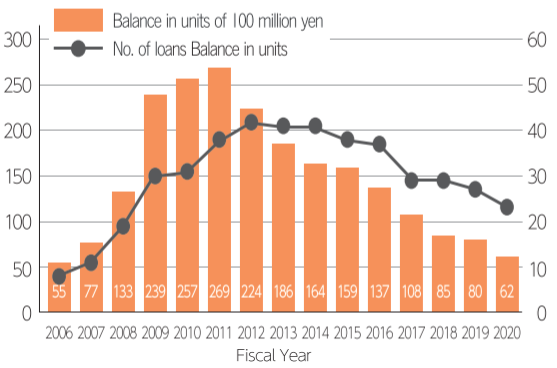
\includegraphics[width=\textwidth]{Images/Metals_policies/JOGMEC1.png}
         \caption{Solde des prêts en cours pour l'exploration à l'étranger}
         \label{fig:JOGMEC1}
    \end{subfigure}
    \hfill
    \begin{subfigure}[b]{0.31\textwidth}
        \centering
         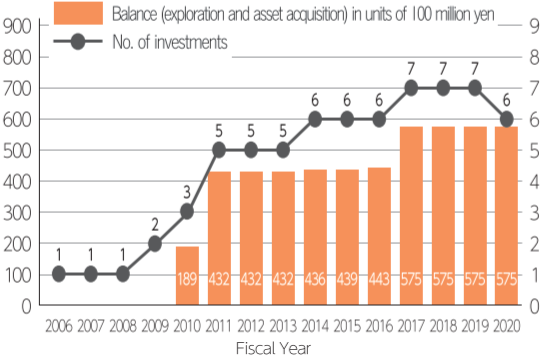
\includegraphics[width=\textwidth]{Images/Metals_policies/JOGMEC2.png}
         \caption{Solde des capitaux propres en circulation}
         \label{fig:JOGMEC2}
    \end{subfigure}
    \hfill
    \begin{subfigure}[b]{0.31\textwidth}
        \centering
         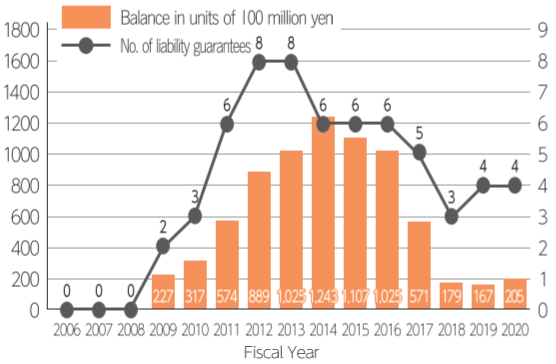
\includegraphics[width=\textwidth]{Images/Metals_policies/JOGMEC3.png}
         \caption{Solde des garanties de passif en cours}
         \label{fig:JOGMEC3}
    \end{subfigure}
    \caption{Activités financières de la JOGMEC}
    \label{fig:metal_histoire}
\end{figure}
~\\
\textbf{Investissements Publics}\smallbreak
Pour développer de nouvelles sources d'approvisionnement, les pays peuvent investir directement dans des fonds publics par le biais d'entreprises publiques, en effectuant des prises de participation publiques dans des entreprises ou des projets privés, ou en utilisant des mécanismes de passation des marchés publics pour acheter la production d'une source spécifique pour les stocks nationaux ou d'autres utilisations gouvernementales.\smallbreak
Le Japon dispose de deux organismes pour diriger des investissements publics vers l'extraction minière : la JOGMEC (Japan Oil, Gas and Metals National Corporation) et la JBIC (Japan Bank for International Cooperation).\smallbreak
La JOGMEC dispose d'un système de participation au capital, de prêts et de garanties de dettes pour les projets de développement de ressources minérales à l'étranger aux stades de l'exploration, du développement et de la production. Ceux-ci, associés au soutien technique de JOGMEC pour le développement de la mine, permettent une réponse de soutien financier flexible. À partir de l'exercice 2020, le budget de JOGMEC comprenait environ 60 milliards JPY (420 millions USD) pour les investissements d'exploration et d'acquisition d'actifs, 6 milliards JPY (40 millions USD) pour les prêts d'exploration et 20 milliards JPY (140 millions USD) en garanties de dette.\smallbreak
La JBIC, quant à elle, dispose d'un système distinct de prêts et de garanties de dettes pour les projets de développement des ressources minérales à l'étranger aux stades de développement et de production. Le principal soutien de JBIC est en tant que prêteur majoritaire dans le financement de projets pour des projets miniers à grande échelle avec un risque technique relativement faible. Les prêts de JBIC sont relativement plus importants que ceux de JOGMEC, avec des prêts allant de dizaines de milliards de yens à des centaines de milliards de yens. La JBIC a également le pouvoir de fournir un soutien financier par le biais d'une participation au capital, mais cela n'a jamais été mis en œuvre (\cite{noauthor_jogmec_2021}).\bigbreak

\textbf{Stocks stratégiques}\smallbreak
Les politiques peuvent être conçues pour prévenir les risques tels que les perturbations de la chaîne d'approvisionnement, les flambées des prix en conservant (et en maintenant) les réserves de minéraux essentiels extraits. Les systèmes de stockage peuvent être associés à des mécanismes de libération déclenchés par des ruptures d'approvisionnement. Cette approche permet par ailleurs de développer un écosystème industriel local autour de métaux. Elle pourrait par exemple offrir des prix garantis de long terme permettant de développer les filières de recyclage (\cite{donnen_vers_2022}).\smallbreak
En mars 2020, le gouvernement japonais a mis à jour la stratégie de gestion de son stock stratégique de métaux. La loi japonaise donne autorité au JOGMEC pour mettre en place un stock stratégique de métaux afin de maintenir un approvisionnement stable en cas de rupture d'approvisionnement. En général, les types de minerai et les quantités spécifiques pour lesquels des stocks sont détenus ne sont pas divulgués, car la divulgation pourrait avoir un impact négatif sur le marché. Pour gérer le stock, JOGMEC subventionne les intérêts nécessaires pour emprunter des fonds pour l'achat de métaux rares et les coûts nécessaires à l'entretien et à la gestion des entrepôts de stockage.\smallbreak
Dans la stratégie de ressources 2020, le gouvernement a annoncé son intention de revoir la façon dont il fixe le volume cible des stocks et de fixer l'objectif en se basant uniquement sur les stocks nationaux - c'est-à-dire sans inclure les stocks de l'industrie. Le nombre cible est généralement fixé à 60 jours, mais pour les minerais à haut risque géopolitique, il pourrait être fixé à un nombre plus élevé « comme 180 jours ».\smallbreak
Outre le stockage, la stratégie des ressources a également annoncé l'intention de renforcer la coopération internationale bilatérale et multilatérale par le biais de JOGMEC et de renforcer le développement technologique pour le recyclage et le développement des matériaux de sous-produits. Parmi les métaux ciblés par le système de stockage on note : le lithium, le cobalt, le nickel, les terres rares.
